\usetikzlibrary{calc,arrows.meta}
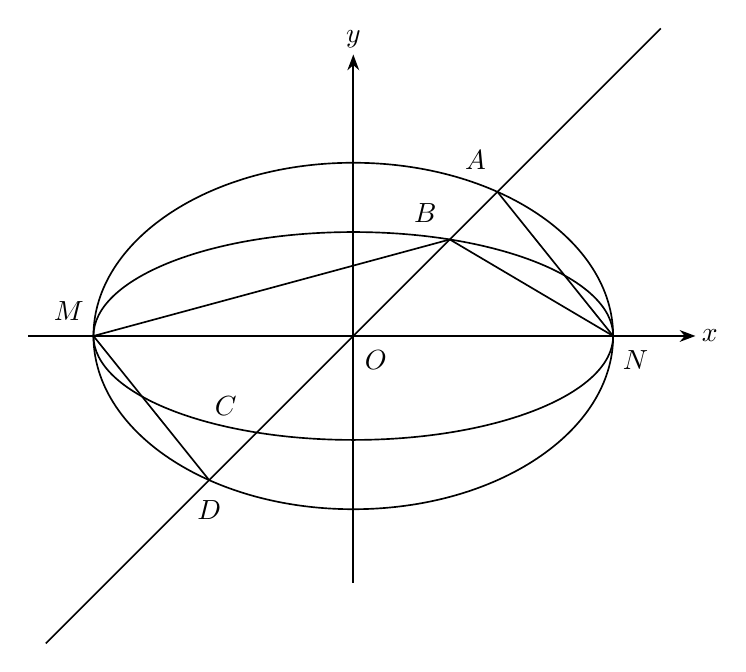
\begin{tikzpicture}[x=1.1cm,y=1.1cm,line width=.6pt,>=Stealth,font=\normalsize]
\coordinate (O) at (0,0);
\coordinate (M) at (-3,0);
\coordinate (N) at (3,0);
\coordinate (A) at (1.6641,1.6641);
\coordinate (B) at (1.1142,1.1142);
\coordinate (C) at (-1.1142,-1.1142);
\coordinate (D) at (-1.6641,-1.6641);
\coordinate (L1) at (-3.55,-3.55);
\coordinate (L2) at (3.55,3.55);
\draw[->] (-3.75,0)--(3.95,0) node[anchor=west,inner sep=0pt,xshift=2pt] {$x$};
\draw[->] (0,-2.85)--(0,3.25) node[anchor=south,inner sep=0pt,yshift=2pt] {$y$};
\draw (O) ellipse [x radius=3, y radius=2];
\draw (O) ellipse [x radius=3, y radius=1.2];
\draw (L1)--(L2);
\draw (M)--(B);
\draw (M)--(D);
\draw (B)--(N);
\draw (A)--(N);
\node[anchor=north west,inner sep=2pt] at ($(O)+(0.06,-0.10)$) {$O$};
\node[anchor=south east,inner sep=2pt] at ($(M)+(-0.04,0.10)$) {$M$};
\node[anchor=north west,inner sep=2pt] at ($(N)+(0.04,-0.10)$) {$N$};
\node[anchor=south east,inner sep=2pt] at ($(A)+(-0.06,0.18)$) {$A$};
\node[anchor=south east,inner sep=2pt] at ($(B)+(-0.08,0.12)$) {$B$};
\node[anchor=south east,inner sep=2pt] at ($(C)+(-0.16,0.12)$) {$C$};
\node[anchor=north,inner sep=2pt] at ($(D)+(0,-0.16)$) {$D$};
\end{tikzpicture}
